\section{Generalising the Charney–Phillips staggering for arbitrary meshes}
\label{sec:cp:method}

The generalisation of the Lorenz staggering for arbitrary meshes is straightforward \citep{weller-shahrokhi2014} but this is not true for the Charney--Phillips staggering, which is only suitable for structured meshes with cells stacked in columns.
On a finite volume mesh, variables are ordinarily placed at cell centres or cell faces.
In the Charney--Phillips staggering, the thermodynamic variable is placed at only those cell faces that lie on the vertical coordinate surfaces, and vertically-oriented faces have no thermodynamic information.
This existing staggering is unsuitable for arbitrary finite volume meshes because faces can have any orientation.

A generalised Charney--Phillips staggering will be particularly relevant to atmospheric models that use vertical mesh refinement techniques.
Mesh refinement has received growing attention in atmospheric modelling literature because it could enable atmospheric models to produce more accurate forecasts with less computation \citep{behrens2006,jablonowski2009}.
While much of the literature concentrates on horizontal mesh refinement, some investigations have been made into vertical refinement on two-dimensional $x$--$z$ Cartesian planes:
\citet{mueller2013} have used conforming refinement of triangular meshes for simulating the standard rising bubble and density current test cases, \citet{vanhooft2018} have used block-structured adaptive mesh refinement for direct numerical simulations of the atmospheric boundary layer, and \citet{yamazaki-satomura2012} have used nonconforming block-refinement to better resolve the atmosphere immediately above idealised mountains.

According to \citet{thuburn-woolings2005}, the vertical discretisation used by \citet{yamazaki-satomura2012} supports computational modes and instabilities, although these errors were not excited by the test cases performed by \citet{yamazaki-satomura2012}.
The Charney--Phillips staggering is not susceptible to such errors, but we are not aware of any existing literature that combines mesh refinement with a Charney--Phillips staggering.
By allowing for an arbitrary mesh, a generalised Charney--Phillips formulation should be suitable for any type of mesh, including conforming and non-conforming mesh refinement, terrain-following meshes, cut cell meshes and slanted cell meshes.

\subsection{Generalised Charney--Phillips formulation}

\begin{figure}
	\centering
	\documentclass[tikz]{standalone}
\usepackage{times}
\usepackage{bm}
\begin{document}
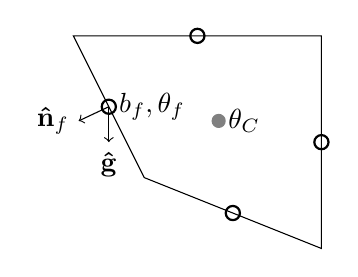
\begin{tikzpicture}[
  scale=0.45,
  cpnt/.style={fill=gray}
]

\draw (2,3) -- (0,7) -- (7,7) -- (7,1) -- (2,3);

\path [cpnt] (4.1,4.6) circle [radius=0.2] node [right] {$\theta_C$};

\draw [thick] (7,4) circle [radius=0.2];
\draw [thick] (4.5,2) circle [radius=0.2];
\draw [thick] (3.5,7) circle [radius=0.2];
\draw [thick] (1,5) circle [radius=0.2] node [right] {$b_f, \theta_f$};

\draw [->] (1,5) -- (0.15,4.6) node [left] {$\mathbf{\hat{n}}_f$};
\draw [->] (1,5) -- (1,4) node [below] {$\mathbf{\hat{g}}$};

\end{tikzpicture}
\end{document}

	\caption{A quadrilateral cell with the prognostic thermodynamic variable $b_f$ stored at face centres marked by open circles.
	$b_f$ is calculated from the potential temperature $\theta_f$ such that $b_f = \theta_f \unitg \cdot \unitn_f$ where $\unitn_f$ is the unit vector outward normal to face $f$, and $\unitg$ is the unit vector of gravitational acceleration.
	The potential temperature at the cell centre, $\theta_C$, is reconstructed from surrounding values of $b_f$ using equation~\eqref{eqn:cp:reconstruct}.}
	\label{fig:cp:staggering}
\end{figure}

The generalised Charney--Phillips model is a new variant of the fully compressible Euler model with a Lorenz staggering, as documented by \citet{weller-shahrokhi2014} and summarised in section~\ref{sec:slanted:exnerFoamH}.
The model variant uses a newly-formulated generalisation of the Charney--Phillips staggering for arbitrary meshes.
The primary difference between the Lorenz and Charney--Phillips formulations is their treatment of the prognostic thermodynamic variable: the generalised Charney--Phillips formulation stores the prognostic thermodynamic variable $b_f$ at all cell faces such that $b_f = \theta_f \unitg \cdot \unitn_f$ where $f$ is a face, $\theta_f$ is the potential temperature at the face, $\unitg$ is the unit vector of gravitational acceleration and $\unitn_f$ is the unit vector that is outward normal to the face.
This arrangement is illustrated in figure~\ref{fig:cp:staggering}.
To transport the thermal field, first, potential temperature is transported in advective form using first-order time-stepping,
\begin{align}
	\theta_f^{n+1} &= \theta_f^n - \Delta t \uf \cdot \left( \nabla_c \theta_f^{\ell} \right)_F \label{eqn:cp:advection}
\end{align}
where $\theta_f^{n+1}$ is the value of $\theta_f$ at the new time-step, $\theta_f^\ell$ is the lagged value from the previous time-stepping iteration, $\uf$ is the velocity, $\left( \cdot \right)_F$ denotes an interpolation from cell centres to faces, and $\nabla_c$ denotes a cell centre gradient \citep{weller-shahrokhi2014}.
Next, $b_f$ is calculated such that $b_f = \theta_f \unitg \cdot \unitn_f$.  
On a Cartesian mesh with no diagonal faces, $b_f$ is zero for entirely vertical faces and $b_f = \theta_f$ for entirely horizontal faces.

Potential temperature at the cell centre is reconstructed from bordering faces,
\begin{align}
	\theta_C &= \unitg \cdot \left( \sum_{f \in c} \unitn_f \Sf \right)^{-1} \cdot \sum_{f \in c} \Sf b_f \label{eqn:cp:reconstruct}
\end{align}
where $\theta_C$ is the reconstructed potential temperature.
On a rectangular Cartesian mesh with no diagonal faces, $\theta_C$ is simply a linear interpolation from the face values immediately above and below the cell centre, and the generalised Charney--Phillips formulation reduces to the standard Charney--Phillips formulation.

Finally, $\theta_f$ is recalculated from $b_f$ and $\theta_C$,
\begin{align}
	\theta_f &:= \Mag{ \unitg \cdot \unitn_f \theta_f} + \left( 1 - \Mag{\unitg \cdot \unitn_f } \right) \left( \theta_C \right)_F \text{.}
\end{align}
This ensures that values of $\theta_f$ on vertical faces is calculated from nearby $b_f$ values and is not retained across time-steps.

The generalised Charney--Phillips model variant makes two other modifications to the Lorenz model variant in order to simplify implementation: first, gravity waves are treated explicitly and, second, first-order Euler semi-implicit time-stepping is used with deferred correction of explicit terms (equation~\ref{eqn:cp:advection}).

